\documentclass[usenames,svgnames,14pt]{beamer}
\usepackage[english]{babel}
\usepackage{
  fontspec,
  fontawesome,
  xcolor,
  mathabx,
  listings,
  lstautogobble,
  TeXnicalities
}

\setsansfont{Yanone Kaffeesatz}[
    UprightFont     = *-Regular ,
    BoldFont        = *-Bold ,
    BoldItalicFont  = *-Bold ,
    BoldSlantedFont = *-Bold ,
    ItalicFont      = *-Light ,
    SlantedFont     = *-Light ,
    SmallCapsFont   = *-Thin
]
\graphicspath{{Figures/}}
\usetheme[style=green]{Z02}

\usetikzlibrary{
    positioning,
    shapes,
}
%Colors for listings
\colorlet{background-color}{gray!20}
\colorlet{basic-color}{black}
\colorlet{keywords-color}{Goldenrod}
\colorlet{comment-color}{red!95!black}
\colorlet{strings-color}{ForestGreen}
\colorlet{builtins-color}{MediumBlue!90!black}
\colorlet{functions-color}{NavyBlue}
\colorlet{variables-color}{DarkOrange}
\colorlet{environment-color}{Gray}
\colorlet{external-color}{SteelBlue}

% https://tex.stackexchange.com/a/34000
\makeatletter
\lst@Key{countblanklines}{true}[t]%
    {\lstKV@SetIf{#1}\lst@ifcountblanklines}

\lst@AddToHook{OnEmptyLine}{%
    \lst@ifnumberblanklines\else%
       \lst@ifcountblanklines\else%
         \advance\c@lstnumber-\@ne\relax%
       \fi%
    \fi}
\makeatother

%listings set
\lstdefinestyle{MyBash}{
backgroundcolor=\color{background-color}, % choose the background color; you must add \usepackage{color} or \usepackage{xcolor}
breakatwhitespace=false,            % sets if automatic breaks should only happen at whitespace
breaklines=true,                    % sets automatic line breaking
captionpos=b,                       % sets the caption-position to bottom
deletekeywords={...},               % if you want to delete keywords from the given language
escapeinside={@|}{|@},              % if you want to add LaTeX within your code
extendedchars=true,                 % lets you use non-ASCII characters; for 8-bits encodings only,
                                    % does not work with UTF-8
frame=single,                       % adds a frame around the code
framerule=0pt,                      % Width of the frame rule
framesep=3pt,                       % separation around text
linewidth=\textwidth,               % defines the base line width for listings
xleftmargin=6mm,                    % Margin left
xrightmargin=6mm,                   % Margin right
numbers=left,                       % where to put the line-numbers; possible values are (none, left, right)
numberblanklines=false,             % suppress numbers on empty lines
countblanklines=false,              % NOT standard! Avoid counting empty lines: https://tex.stackexchange.com/a/34000
numbersep=8pt,                      % how far the line-numbers are from the code
numberstyle=\tiny\color{black},     % the style that is used for the line-numbers
rulecolor=\color{black},            % if not set, the frame-color may be changed on line-breaks within not-black text
                                    % (e.g. comments (green here))
showspaces=false,                   % show spaces everywhere adding particular underscores; it overrides 'showstringspaces'
showstringspaces=false,             % underline spaces within strings only
showtabs=false,                     % show tabs within strings adding particular underscores
stepnumber=1,                       % the step between two line-numbers. If it's 1, each line will be numbered
tabsize=2,                          % sets default tabsize to 2 spaces
title=\lstname,                     % show the filename of files included with \lstinputlisting; also try caption instead of title
%
%Base style for this presentation 
keepspaces=true,                    % keeps spaces in text, useful for keeping indentation of code
                                    % (possibly needs columns=flexible)
language=bash,
basicstyle=\ttfamily\scriptsize\color{basic-color},
keywordstyle=\color{keywords-color},
stringstyle=\color{strings-color},
commentstyle=\color{comment-color},
morestring=[b][\color{strings-color}]{"},
morestring=[d][\color{strings-color}]{'},
moredelim=[is][\color{basic-color}]{|+}{+|}, % I will use this for terminal output
literate={`}{\textasciigrave}1, % https://tex.stackexchange.com/a/466224/128737
literate={~}{{\textasciitilde}}1,
% literate=% literate={<replace>}{<replacement text>}{<width>}
%   {\#define}{{{\color{CarnationPink}\#define}}}{6}
%   {\#include}{{{\color{CarnationPink}\#include}}}{7},
alsoletter=0123456789![]/\{\}.:+, % This to mark the symbols in keyword/emph[5] to be highlighted (otherkeywords does not work i.e. it highlights also in comments!) -> manual at page 45
morekeywords={if, then, else, elif, fi, case, esac, for, select, while, until, do, done, in, function, time, [[, ]], \{, \}, !, coproc}, %https://askubuntu.com/a/513712
emph=[1]{},
emphstyle=[1]{\color{functions-color}}, %Functions
emph=[2]{},
emphstyle=[2]{\color{variables-color}}, %Variables
emph=[4]{PATH, SHELL, IFS, BASH_ALIASES, BASH_REMATCH, PS3, REPLY, HOME, LANGUAGE, EDITOR, PIPESTATUS, PWD, FUNCNEST,
         DIRSTACK, PWD, OLDPWD, SHELLOPTS, BASHOPTS, TIMEFORMAT, COMP_CWORD, COMP_LINE, COMP_POINT, COMP_TYPE, COMP_KEY,
         COMP_WORDBREAKS, COMP_WORDS, COMPREPLY, INPUTRC},
emphstyle=[4]{\color{environment-color}}, %Environment variables
emph=[5]{alias, bg, bind, break, builtin, cd, command, compgen, complete, continue, declare, dirs, disown, echo, enable, eval,
         exec, exit, export, false, fc, fg, getopts, hash, help, history, jobs, kill, let, local, logout, popd, printf, pushd, pwd,
         read, readonly, return, set, shift, shopt, source, suspend, test, times, trap, true, type, typeset, ulimit, umask,
         % case, if, until, while  % <--- these built-in are keywords and I leave them highlighted as such
         unalias, unset, wait, :, ., [, ]},
emphstyle=[5]{\color{builtins-color}}, %Shell built-in
emph=[6]{man, apropos, ls, rm, g++, chmod, cp, awk, sed, cut, perl, args, date, grep, sleep, tput, seq, cat, wc, sort, uniq, tail,
         head, sdiff, tar, mktemp, mkdir, ps, emacs, systemd, timeout, parallel, xargs, gnuplot, pdflatex, vi, ping, bash,
         egrep, shuf, stat, find, fgrep, bc, tr, paste, expr, diff, touch},
emphstyle=[6]{\color{external-color}}, %(External) commands
emph=[7]{},
emphstyle=[7]{\color{variables-color}}, %Class for local variables (usually with bad names)
emph=[8]{},
emphstyle=[8]{\color{builtins-color}}, %Class for local commands (usually with bad names)
%
%Additional customizations
belowskip=-7mm,
aboveskip=3pt,
autogobble=true, % lstautogobble needed!
}

\lstnewenvironment{Bash}[1][] %I will rarely use this because putting a $ in it as prompt breaks down TeXclipse highlight syntax!
    {\lstset{style=MyBash, #1}}
    {}

\def\bash{\lstinline[style=MyBash, basicstyle=\ttfamily\color{black}]}


%===============================================================%
\title{Introduction to Git}
\author{Alessandro Sciarra}
\institute{Z02~--~Software Development Center}
\titlegraphic{
\includegraphics[width=20mm]{LogoCRC}}
\titlepagelogo{
\includegraphics[width=20mm]{LogoGoethe}}
%===============================================================%

\AtBeginSection[] % <- Empty optional argument, do nothing for \section*
{
    \begin{frame}[plain, noframenumbering]{}
         \sectionpage
    \end{frame}
}

\begin{document}

%===============================================================%
\begin{frame}[plain,noframenumbering]
    \titlepage
\end{frame}
%~~~~~~~~~~~~~~~~~~~~~~~~~~~~~~~~~~~~~~~~~~~~%
\begin{frame}{Outline of the talk}
    \tableofcontents[subsectionstyle=hide]
\end{frame}
%===============================================================%


%===============================================================%
\section{Why should you use it?}
%~~~~~~~~~~~~~~~~~~~~~~~~~~~~~~~~~~~~~~~~~~~~%
\AlertFrame{OK, let's do it without git}
%~~~~~~~~~~~~~~~~~~~~~~~~~~~~~~~~~~~~~~~~~~~~%
\begin{frame}{A possible workflow}{Writing a review or a Ph.D. thesis}
    \vspace{-0.1\textheight}
    \begin{tikzpicture}[remember picture, overlay]
        \node[anchor=east, visible on=<+>, inner xsep=5mm] at (current page.east) {
\includegraphics[width=0.55\textwidth]{FinalDoc}};
    \end{tikzpicture}
    \setlength{\leftmarginii}{0.5cm}
    \begin{overlayarea}{\textwidth}{0.5\textheight}
        \begin{itemize}
            \item<+-> \textcolor<.-.(1)>{PQ}{How do you make writing experiments?}
                  \par\begin{onlyenv}<+> % <------ the \par is to avoid vertical shift: https://tex.stackexchange.com/a/449826
                      \begin{itemize}
                          \item You make a backup of your file
                          \item You comment out a block of text in your source
                          \item If the old version was better, you restore by hand
                          \item If the new version is better, you clean by hand
                      \end{itemize}
                  \end{onlyenv}
            \item<+-> \textcolor<.-.(1)>{PQ}{How do you create/view checkpoints?}
                  \par\begin{onlyenv}<+>
                      \begin{itemize}
                          \item Create a .tar or .zip file
                          \item Copy it somewhere and uncompress if needed
                      \end{itemize}
                  \end{onlyenv}
            \item<+-> \textcolor<.-.(1)>{PQ}{Which version did you send to your supervisor/colleagues?}
                  \par\begin{onlyenv}<+>
                      \begin{itemize}
                          \item Put a copy of the PDF file or of the compressed folder somewhere
                          \item Keep the sent email for later use
                      \end{itemize}
                  \end{onlyenv}
            \item<+-> \PQ{How long did it take to write this section?}
            \item<.-> \PQ{When did I start writing this chapter?}
            \item<.-> \PQ{How much did I write on average per day?}
        \end{itemize}
    \end{overlayarea}
    \begin{varblock}{alert}[0.88\textwidth]{}<+>
        \large\alert{\textbf{Everything by hand, error-prone and big overhead!}}
    \end{varblock}
\end{frame}
%~~~~~~~~~~~~~~~~~~~~~~~~~~~~~~~~~~~~~~~~~~~~%
\begin{frame}{Another possible workflow}{Collaborating on a project}
    \setlength{\leftmarginii}{0.5cm}
    \begin{overlayarea}{\textwidth}{0.6\textheight}
        \begin{itemize}
            \item<+-> \textcolor<.-.(1)>{PQ}{How can you work on the same project?}
                    \par\begin{onlyenv}<+> % <------ the \par is to avoid vertical shift: https://tex.stackexchange.com/a/449826
                        \begin{itemize}
                            \item You work on separate parts at the same time
                            \item Only one person works at the same time
                        \end{itemize}
                    \end{onlyenv}
            \item<+-> \textcolor<.-.(1)>{PQ}{How do you merge work from other people in the team?}
                    \par\begin{onlyenv}<+>
                        \begin{itemize}
                            \item You send the changed files per email and put them in the folder by hand
                            \item Copy/Rsync in some shared place the new status of the project
                            \item If only one person at once works, a compressed archive can be exchanged
                        \end{itemize}
                    \end{onlyenv}
            \item<+-> \textcolor<.-.(1)>{PQ}{How do you work on different machines?}
                    \par\begin{onlyenv}<+>
                        \begin{itemize}
                            \item You don't, use \texttt{SSH}
                            \item Different machines are as different people, see above
                        \end{itemize}
                    \end{onlyenv}
            \item<+-> \textcolor<.-.(1)>{PQ}{How do you know who did what?}
                    \par\begin{onlyenv}<+>
                        \begin{itemize}
                            \item This information is not important
                            \item Sending work around per email allows to trace this\ldots
                            \item Put comments into the source!
                        \end{itemize}
                    \end{onlyenv}
            \item<+-> \textcolor<.-.(1)>{PQ}{How do you give credit to authors?}
                    \par\begin{onlyenv}<+>
                        \begin{itemize}
                            \item Detailed information is not important
                            \item A rough idea about who worked on what is enough
                            \item See comments into the source!
                        \end{itemize}
                    \end{onlyenv}
            \item<+-> \textcolor<.-.(1)>{PQ}{How do you go back in history e.g.\ in case of a bug?}
                    \par\begin{onlyenv}<+->
                        \begin{itemize}
                            \item Again, use the archive sent around per email
                            \item Using a shared place, this is not possible $\;\to\;$ debug!
                        \end{itemize}
                    \end{onlyenv}
        \end{itemize}
    \end{overlayarea}
    \begin{tikzpicture}[remember picture, overlay]
        \node[anchor=north east, visible on=<+>, inner xsep=5mm, inner ysep=2mm] at (current page.north east) {
\includegraphics[width=0.3\textwidth]{Head-explosion}};
    \end{tikzpicture}
\end{frame}
%~~~~~~~~~~~~~~~~~~~~~~~~~~~~~~~~~~~~~~~~~~~~%
\AlertFrame{OK, and how would it be with Git?}
%~~~~~~~~~~~~~~~~~~~~~~~~~~~~~~~~~~~~~~~~~~~~%
\begin{frame}{A possible workflow}{Writing a review or a Ph.D. thesis}
    %\vspace{-0.1\textheight}
    \setlength{\leftmarginii}{0.5cm}
    \begin{customlist}{5mm}
        \item How do you make writing experiments?
              \begin{itemize}
                  \item Just do them (staging/stash area)
                  \item \texttt{git-branch}
              \end{itemize}
        \item How do you create/view checkpoints?
              \begin{itemize}
                  \item \texttt{git-log} \quad \texttt{git-tag} \quad \texttt{git-checkout}
              \end{itemize}
        \item Which version did you send to your supervisor/colleagues?
              \begin{itemize}
                  \item \texttt{git-log} \quad \texttt{git-tag}
              \end{itemize}
        \item How long did it take to write this section?\tikzmark{start}
        \item When did I start writing this chapter?
        \item How much did I write on average per day?\tikzmark{end}
    \end{customlist}
    \CurlyRemark{start}{end}[font=\ttfamily\small]{git-shortlog\\ git-log\\ gitstats$^\star$}
    \FrameRemark{$^\star$ This is just one of the pletora of libraries to make statistics based on a git repository.}
\end{frame}
%~~~~~~~~~~~~~~~~~~~~~~~~~~~~~~~~~~~~~~~~~~~~%
\begin{frame}{Another possible workflow}{Collaborating on a project}
    \setlength{\leftmarginii}{0.5cm}
    \begin{customlist}{5mm}
        \item How can you work on the same project?
              \begin{itemize}
                  \item \texttt{git-pull} \quad \texttt{git-push} \quad \texttt{git-branch}
              \end{itemize}
        \item How do you merge work from other people in the team?
              \begin{itemize}
                  \item \texttt{git-merge}
              \end{itemize}
        \item How do you work on different machines?
              \begin{itemize}
                  \item \texttt{git-pull} \quad \texttt{git-push}
              \end{itemize}
        \item How do you know who did what?
              \begin{itemize}
                  \item \texttt{git-blame}
              \end{itemize}
        \item How do you give credit to authors?
              \begin{itemize}
                  \item \texttt{git-shortlog}
              \end{itemize}
        \item How do you go back in history e.g.\ in case of a bug?
              \begin{itemize}
                  \item \texttt{git-checkout} \quad \texttt{git-bisect}
              \end{itemize}
    \end{customlist}
\end{frame}
%~~~~~~~~~~~~~~~~~~~~~~~~~~~~~~~~~~~~~~~~~~~~%
\begin{frame}{Yes, but I have to learn all those commands!}
    \begin{onlyenv}<1>
        \begin{center}
            \tikzmark{figureStart}There are many jokes on the web\ldots\\[1ex]
            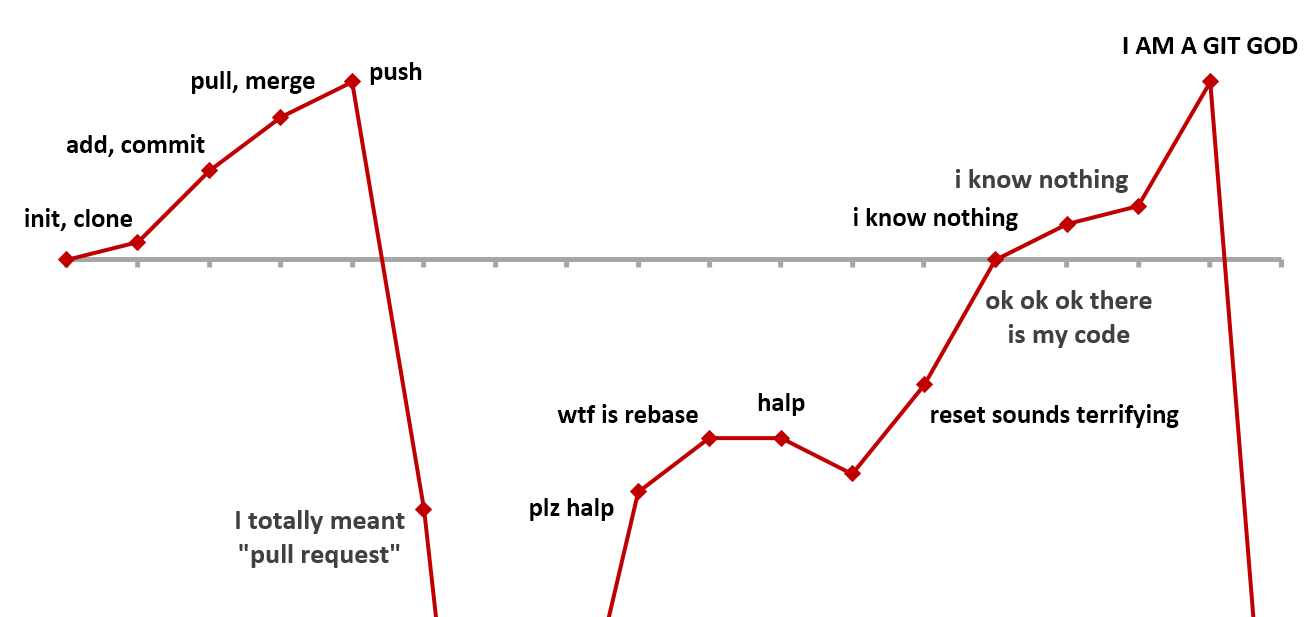
\includegraphics[width=0.75\textwidth]{Git-learning-curve}\\[2ex]
            \PB{\ldots{}but after all it is about having the correct mental set up!}
        \end{center}
        \begin{tikzpicture}[remember picture, overlay]
            \coordinate (center) at ($(figureStart)-(2.5mm,15mm)$);
            \draw[thick, PS, rotate around={30:(center)}] (center) ellipse (18mm and 8mm);
            \node[font=\small, text=PS, anchor=west] at ($(figureStart)+(14mm,-8mm)$) {This makes sense};
        \end{tikzpicture}
    \end{onlyenv}
    \begin{onlyenv}<2>
        \begin{itemize}
            \item As any new tool, it needs some practice
            \item \alert{The short- to long-term payoff is worth the effort}
            \item It is plenty of \URL[PP]{https://git-scm.com/downloads/guis/}{GUI clients}
                  \begin{itemize}
                      \item \URL[PB]{https://www.sourcetreeapp.com/}{Sourcetree:} A Free GIT Client For Windows And Mac
                      \item \URL[PB]{https://aurees.com/}{Aurees:} Easy-Fast-Free \Remark{Windows, Mac \& Linux}
                      \item \URL[PB]{https://git-cola.github.io/}{Git-Cola:} Powerful GUI For GIT \Remark{Windows, Mac, Ubuntu \& Linux}
                      \item{} [\ldots]
                  \end{itemize}
            \item You can work in the terminal\\ $\,\to\,$ after this (and next) talk it will be possible!
        \end{itemize}
    \end{onlyenv}
    \FrameRemark{Git was not designed to be user-friendly, but it is by far the most used version control system in the world.}
\end{frame}
%~~~~~~~~~~~~~~~~~~~~~~~~~~~~~~~~~~~~~~~~~~~~%
\begin{frame}{Last but not least}
    \vspace{0.05\textheight}
    \begin{varblock}{}[0.95\textwidth]{Which large famous products are developed using Git?}
        Linux, Homebrew, Windows, Tensorflow, Angular, Inkscape, \ldots
    \end{varblock}
    \begin{varblock}{alert}[0.95\textwidth]{And if I do not have so large projects?}<2->
        It doesn't matter!
        There are too many advantages having a writing or coding project under a source code management tool.
        Even alone.
        \textbf{Simply use one (Git).}
        \alert{\textbf{Now.}}
    \end{varblock}
    \vspace{-0.02\textheight}
    \begin{varblock}{alert}[0.95\textwidth]{}<3>
        \small
        For collaborative projects like maintaining code in a group, handing it over from person to person and so on, Git is simply a must.
        \textbf{As project leader, you should think about requiring everybody to work in a Git repository.}
    \end{varblock}
    \begin{tikzpicture}[remember picture, overlay]
        \node[anchor=north east, inner xsep=8mm, inner ysep=3mm] at (current page.north east) {
\includegraphics[width=0.25\textwidth]{Git-Logo}};
    \end{tikzpicture}
\end{frame}
%===============================================================%

%===============================================================%
\section{What is Git?}
%~~~~~~~~~~~~~~~~~~~~~~~~~~~~~~~~~~~~~~~~~~~~%
\begin{frame}{How does Git define itself?}
    \PrepareURLsymbol[PB]
    \begin{varblock}{quote}[0.95\textwidth]{}[\URL*{https://git-scm.com/}{Git homepage}]
        \guillemotleft
        Git is a free and open source distributed version control system designed to handle everything from small to very large projects with speed and efficiency.
        Git is easy to learn and has a tiny footprint with lightning fast performance.\guillemotright
        %It outclasses SCM tools like Subversion, CVS, Perforce, and ClearCase with features like cheap local branching, convenient staging areas, and multiple workflows.
    \end{varblock}
    \begin{enumerate}
        \item Free and open
        \item \textbf{Distributed version control system}
        \item \PP{From small to very large projects}
        \item With speed and efficiency
        \item \alert{Easy to learn}
    \end{enumerate}
\end{frame}
%===============================================================%

%===============================================================%
\section{How does it work?}
%~~~~~~~~~~~~~~~~~~~~~~~~~~~~~~~~~~~~~~~~~~~~%
\begin{frame}{C}
    
\end{frame}
%===============================================================%


\end{document}
